 
\section{Application: Newton's method}\footnote{This section was 
modified from the Wikipedia entry \cite{N}.}
\label{sec:newtons-method}

Newton's method (also known as the Newton–Raphson method) is an 
efficient algorithm for finding approximations to the zeros (or roots) 
of a real-valued function. As such, it is an example of a root-finding 
algorithm. It produces iteratively a sequence of approximations to the 
root. It can also be used to find a minimum or maximum of such a 
function, by finding a zero in the function's first derivative.


\subsection{Description of the method}

The idea of the method is as follows: one starts with an initial 
guess which is reasonably close to the true root, then the function 
is approximated by its tangent line (which can be computed using 
the tools of calculus), and one computes the x-intercept of this 
tangent line (which is easily done with elementary algebra). 
This x-intercept will typically be a better approximation to 
the function's root than the original guess, and the method can be 
iterated.

Suppose $f : [a, b] \to \rrr$ is a differentiable function defined 
on the interval $[a, b]$ with values in the real numbers $\rrr$. The 
formula for converging on the root can be easily derived. 
Suppose we have some current approximation $x_n$. Then we can derive 
the formula for a better approximation, $x_{n+1}$ by referring to 
the diagram on the right. We know from the definition of the 
derivative at a given point that it is the slope of a tangent at that point.

That is

\[
    f'(x_{n}) 
= \frac{ \mathrm{rise} }{ \mathrm{run} } 
= \frac{ \mathrm{\Delta y} }{ \mathrm{\Delta x} } 
= \frac{ f( x_{n} ) - 0 }{ x_{n} - x_{n+1} } 
= \frac{0 - f(x_{n})}{(x_{n+1} - x_{n})}\,\!.
\]
Here, $f'$ denotes the derivative of the function $f$. Then by 
simple algebra we can derive

\[
    x_{n+1} = x_n - \frac{f(x_n)}{f'(x_n)}\,\!. 
\]
We start the process off with some arbitrary initial value $x_0$. 
(The closer to the zero, the better. But, in the absence of any 
intuition about where the zero might lie, a ''guess and check'' 
method might narrow the possibilities to a reasonably small 
interval by appealing to the intermediate value theorem.) The 
method will usually converge, provided this initial guess is close 
enough to the unknown zero, and that $f'(x_0) \neq 0$. Furthermore, 
for a zero of multiplicity $1$, the convergence is at least 
quadratic (see rate of convergence) in a neighbourhood of the 
zero, which intuitively means that the number of correct digits 
roughly at least doubles in every step. More details can be found 
in the analysis section below.

\begin{example}
{\rm
Consider the problem of finding the positive number $x$ with 
$\cos(x) = x^3$. We can rephrase that as finding the zero of 
$f(x) = \cos(x) - x^3$. We have $f'(x) = -\sin(x) - 3x^2$. 
Since $\cos(x) \leq 1$ for all $x$ and $x^3 > 1$ for $x>1$, 
we know that our zero lies between $0$ and $1$. We try a starting 
value of $x_0 = 0.5$.

\[
\begin{array}{lllll} 
x_1 & = & x_0 - \frac{f(x_0)}{f'(x_0)} & 
= & 0.5 - \frac{\cos(0.5) - 0.5^3}{-\sin(0.5) - 3 \times 0.5^2} =  1.112141637097 \\ 
x_2 & = & x_1 - \frac{f(x_1)}{f'(x_1)} & = & \underline{0.9}09672693736 \\ 
x_3 &= & x_2 - \frac{f(x_2)}{f'(x_2)} & = & \underline{0.86}7263818209 \\ 
x_4 &= & x_3 - \frac{f(x_3)}{f'(x_3)} & = & \underline{0.86547}7135298 \\ 
x_5 &= & x_4 - \frac{f(x_4)}{f'(x_4)} & = & \underline{0.8654740331}11 \\ 
x_6 &= & x_5 - \frac{f(x_5)}{f'(x_5)} & = & \underline{0.865474033102} 
\end{array}
\]

The correct digits are underlined in the above example. In 
particular, $x_6$ is correct to the number of decimal places 
given. We see that the number of correct digits after the 
decimal point increases from $2$ (for $x_3$) to $5$ and $10$, 
illustrating the quadratic convergence.
}
\end{example}

\subsection{Analysis}

Suppose that the function $f$ has a zero at $a$, i.e., $f(a) = 0$.

If $f$ is continuously differentiable and its derivative does not vanish 
at $a$, then there exists a neighborhood of $a$ such that for 
all starting values $x_0$ in that neighborhood, the sequence 
$\{x_n\}$ will converge to $a$.

In practice this result is ``local'' and the neighborhood of 
convergence is not known a priori, but there are also some results 
on ``global convergence.'' For instance, given a right neighborhood 
$U$ of $a$, if $f$ is twice differentiable in $U$ and if 
$f' \ne 0$, $f \cdot f'' > 0$ in $U$, then, for each $x_0\in U$ the 
sequence $x_k$ is monotonically decreasing to $a$.

\subsection{Fractals}


For complex functions $f:\ccc\to\ccc$, however, Newton's method can be directly applied 
to find their zeros. For many complex functions, the boundary of the 
set (also known as the basin of attraction) of all starting values
that cause the method to converge to a particular zero is a 
fractal\footnote{The definition of a fractal would take us too far afield.
Roughly speaking, it is a geometrical object with
certain self-similarity properties \cite{F}.}

For example, the function $f(x)=x^5-1$, $x\in \ccc$, has five roots,
equally spaced around the unit circle in the complex plane.
If $x_0$ is a starting point which converges to the root at $x=1$, color $x_0$ yellow.
Repeat this using four other colors (blue, red, green, purple)
for the other four roots of $f$. 
The resulting image is in Figure \ref{fig:newtons-fractal}.

\begin{figure}[h!]
%\begin{tabular}{cc}
\begin{minipage}{\textwidth}
\begin{center}
%\vspace{1.0 cm}
%
\includegraphics[height=4cm,width=4cm]{circle-example.eps}
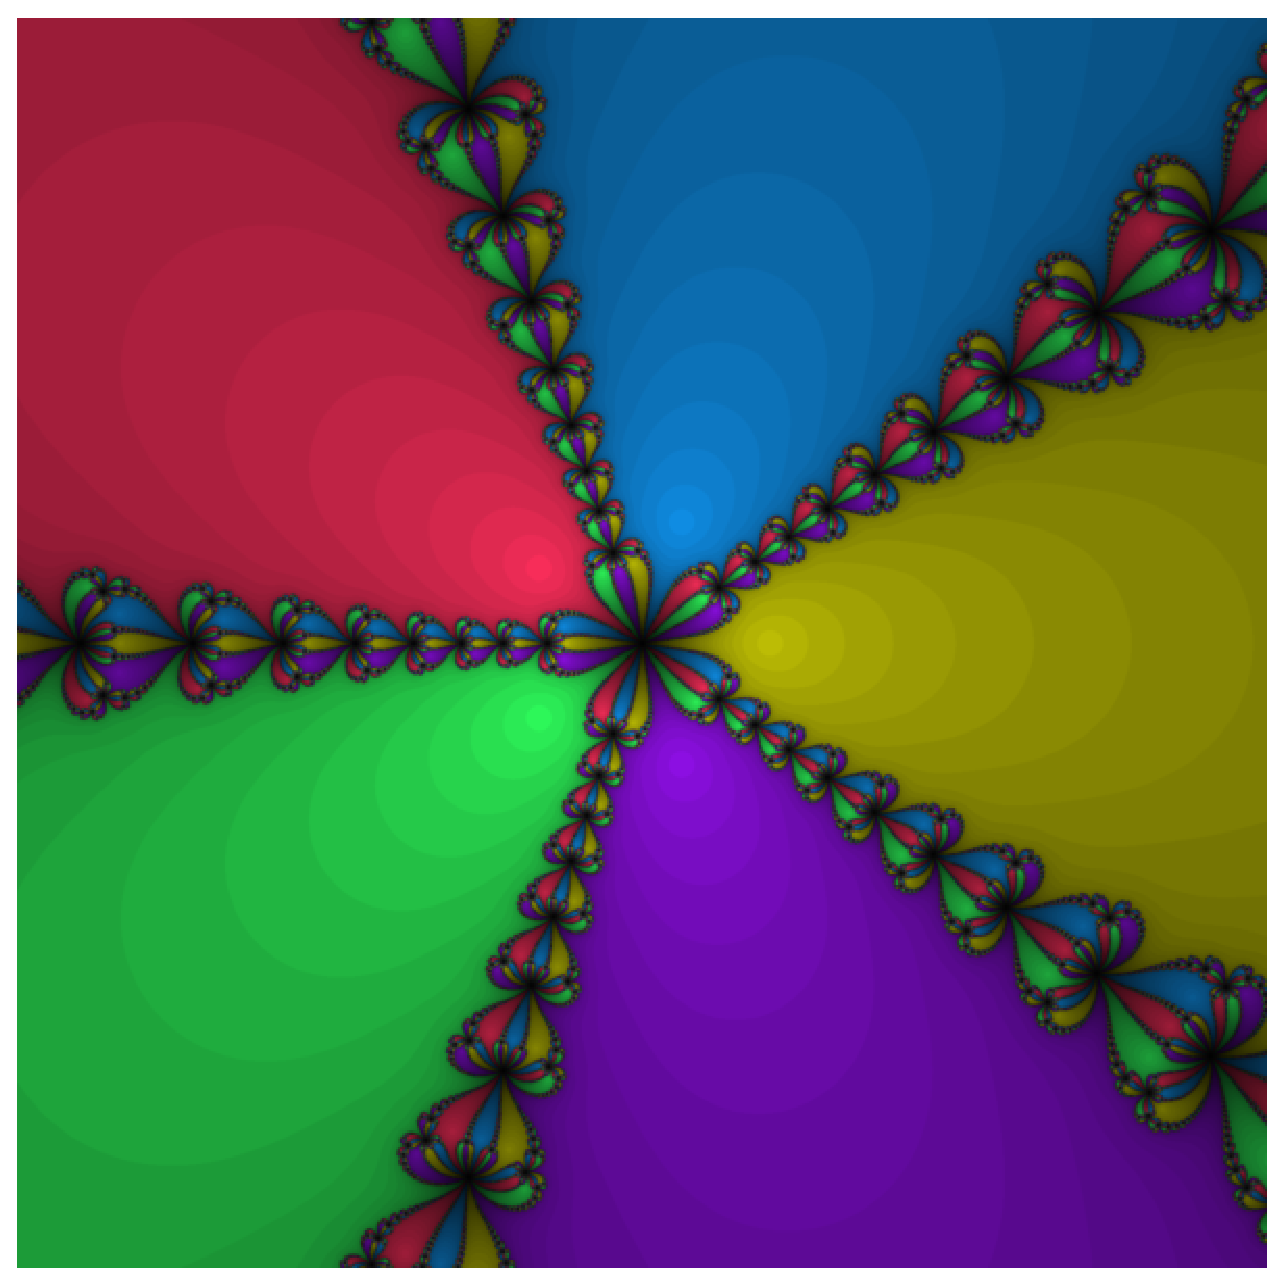
\includegraphics[height=9cm,width=9cm]{newtons-fractal.eps}
\end{center}
\end{minipage}
%\caption{Scan of Granville's graphic of an inscribed circle with rectangle.}
\caption{Basins of attraction for $x^5 - 1 = 0$; darker means more iterations to converge.}
\label{fig:newtons-fractal}
\end{figure}

